\chapter{Amplifier Circuits}
\textit{Amplifiers circuits} \cite{amplifier-circuit} are circuits which increases an electrical input signal according
to a specific transformation function (gain) for each different topology on the output. The circuit for small input signals
normally is composed by an operational amplifier, resistors, trimmer potentiometers to adjust the gain and capacitors.\\

It was required by the project an amplifier which have a gain of 100 ad should be possible to supply with a sigle supply, ideally 5V provided by
the USB port. The circuit should be compact to be a product differential, when compared to the existent systems which needs to connect on greater modules
to perform the same action as the proposed on this project.

It was researched some types of amplifiers circuits on \textit{book} \cite{Milmann} and on \textit{supplier catalogue} \cite{OpAmps}.
After verify some amplifiers topologies it was selected two different circuits which attends the project requirements.
The first circuit uses the Texas Instruments INA 326
Instrumental Amplifier and the second uses the Texas Instruments TLV 4316 Operational Amplifier. These topologies are possible to use with
single supply of 5V and the reach the desirable gain value without distortion on the project frequency range of work (audible frequency range).

\section{INA 326}
The project using the INA 326 IC, started with a research at the \textit{component datasheet} \cite{INA326}
of this component and the \textit{supplier catalogue} \cite{OpAmps}. On theses documents it was verified
the circuit topology \autoref{INA_topology} which provides the desired Gain to
the electric signal from the pickup respecting the project's initial requests.

\begin{figure}[!htpb]
\centering
\caption{INA 326 topology}
\label{INA_topology}
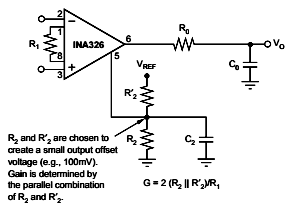
\includegraphics[scale=1]{images/Texas_INA}
\legend{Source: \citeonline{INA326}}
\end{figure}

This circuit amplifies the input signal and the gain is obtained by the following equation \autoref{INA_Gain} provided by the \textit{component datasheet}
\cite{INA326}:

\begin{equation}
\label{INA_Gain}
G=2*\frac{(R_2||R_2 ')}{R_1}
\end{equation}

On the project the Resistor $R_0$ and the Capacitor $C_0$ was excluded because
it was not relevant on the output to this project. It was calculated the values
for the components and then developed a schematic model to perform some simulation tests
to verify the functionalism of the circuit for the desired application.
The schematic circuit \autoref{INA_Schematic} was developed using the software CadSoft Eagle Professional 7.6.0
until the final version.

\begin{figure}[!htpb]
\centering
\caption{INA 326 Schematic Circuit}
\label{INA_Schematic}
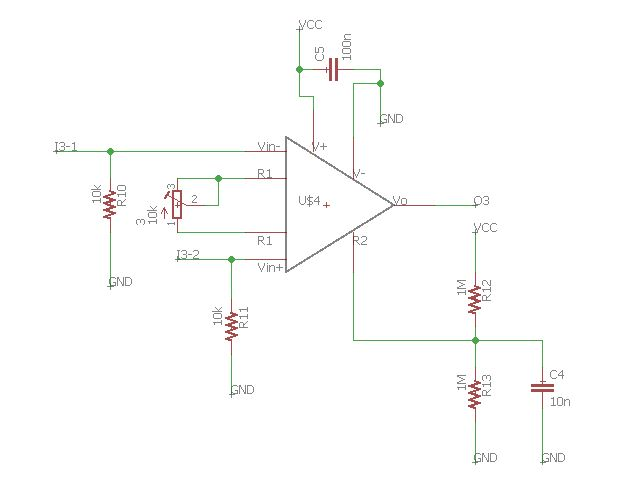
\includegraphics[scale=0.65]{images/INA_Schematic}
\legend{Source: made by authors}
\end{figure}

Using the components values showed on the circuit \autoref{INA_Schematic} it is possible calculate
the Gain of the circuit as the equation\autoref{Gain} shows

\begin{equation}
  \label{Gain}
G=2*\frac{(1M\Omega||1M\Omega)}{10k\Omega}\\
G=2*\frac{500k\Omega}{10k\Omega}\\
G=2*50\\
G=100
\end{equation}

The amplifier circuit was projected to each channel as showed on \autoref{INA_complete}.
So the circuit needed 6 IC INA 326 to be complete.  After project
the schematic circuit to each channel it was developed the PCB project, using the
same software described on the schematic modeling. The PCI project \autoref{INA_PCB}\\

This PCB project was projected on a dual layer board scheme, using 15 mils of
minimum width for the conductive tracks. It was assembled on FR4 dual layer copper
board, combining the through-hole and surface-mount technologies. This choice was
made due the facility of the assembly of the through-hole components and the availability
of the IC only on surface (SOP-8) encapsulation. It was sent
the files to one person who works with printing PCB boards. After the processes
the PCB was like showed on \autoref{PCB}.\\

\begin{figure}[!htpb]
\centering
\caption{Projected INA PCB}
\label{INA_PCB}
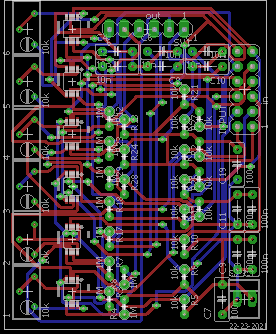
\includegraphics[scale=1.5]{images/TCC_INA}
\legend{Source: made by authors}
\end{figure}

\begin{figure}[!htpb]
\centering
\caption{PCB Project}
\label{INA_PCB}
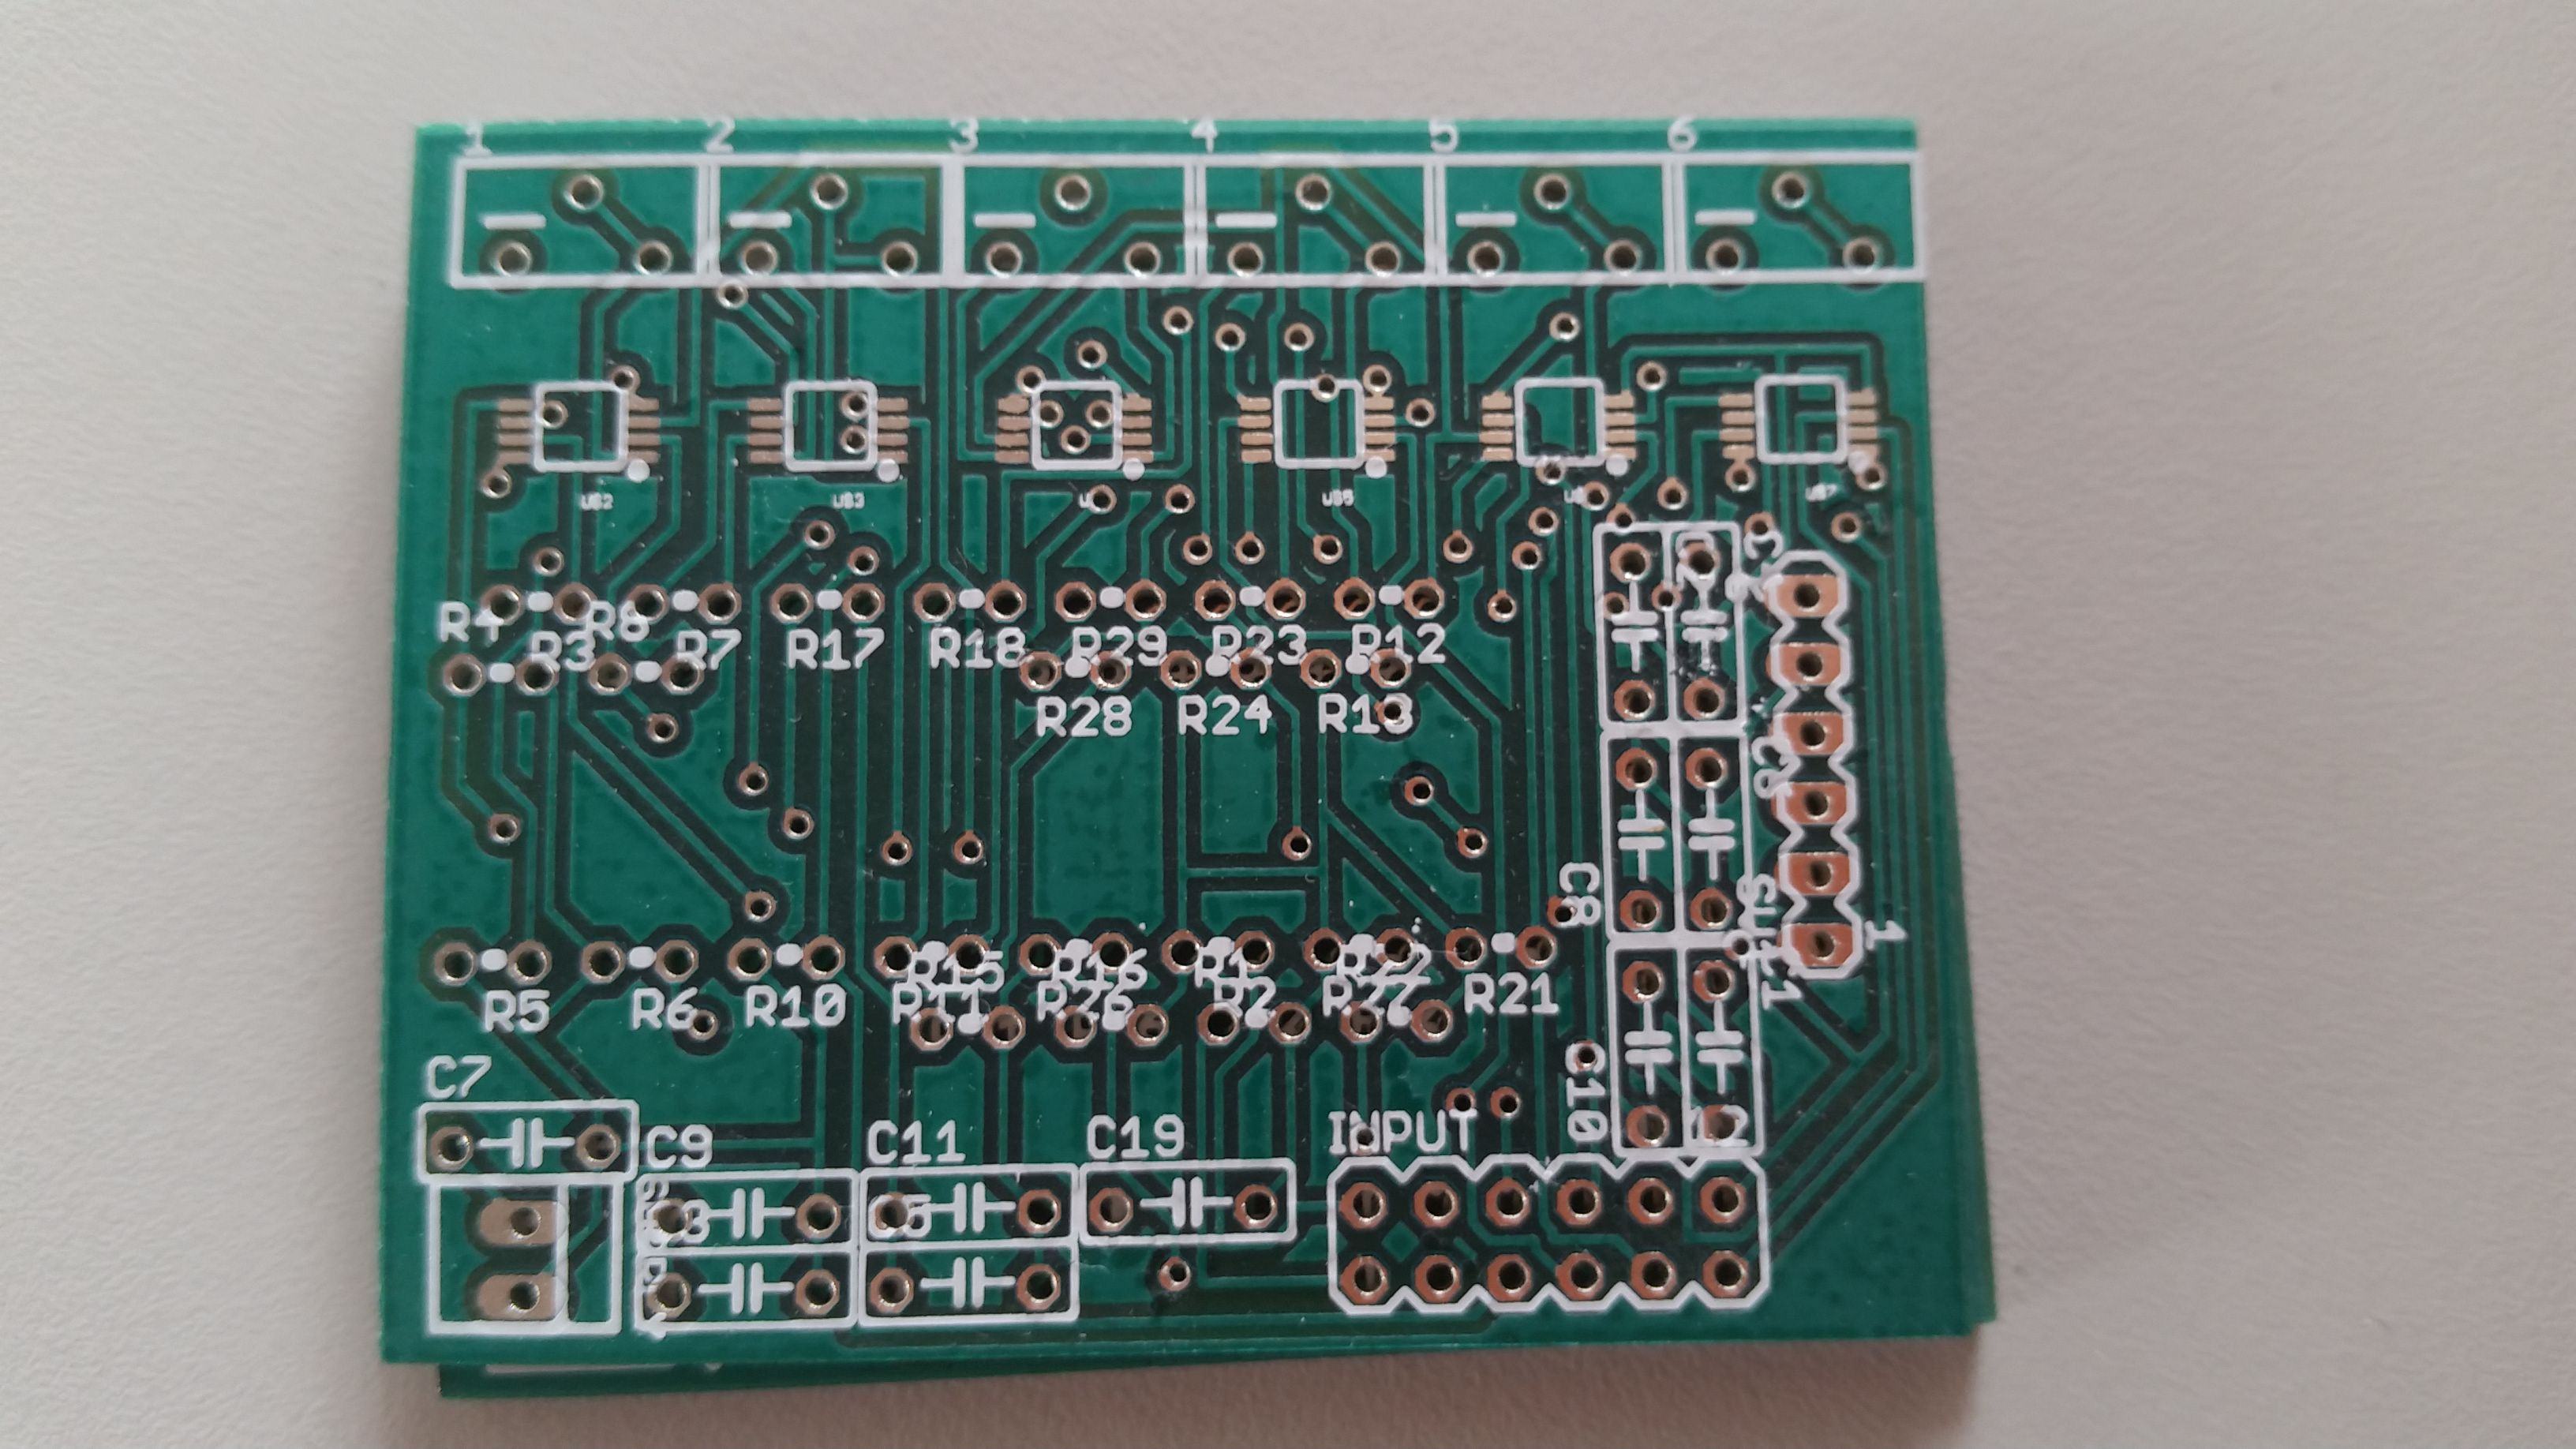
\includegraphics[scale=0.08]{images/INA_board}
\legend{Source: made by authors}
\end{figure}

On this project it was used:

\begin{itemize}
\item 6 Instrumental Amplifiers INA 326;
\item 6 10k$\Omega$ Trimmer Potentiometer;
\item 6 10nF Ceramic Capacitor;
\item 6 100nF x 50V Electrolytic Capacitor;
\item 12 10k$\Omega$ 5 Percent Tolerance Resistor;
\item 12 1M$\Omega$ 5 Percent Tolerance Resistor;
\item 1 6 positions Pin bar;
\item 1 12 positions dual track Pin bar;
\item 1 2 positions Pin bar;
\end{itemize}

After soldering all the components it was performed some bench tests to
verify the functionality of the amplifier circuit. The result showed that the
circuit attends the required function, amplifying the signal from a pick of 10mV
to a pick of 1V, proving that the circuit is working perfectly and attending the
demand of the project. After the bench test the system was connected to the pickup
to verify if the guitar signal would be amplified as needed to the conversion process.
The result was satisfactory and attended well the purpose to the project, as showed on \autoref{INA_result}.

\begin{figure}[!htpb]
\centering
\caption{Amplified pickup signal}
\label{INA_result}
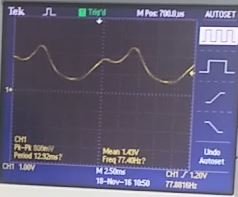
\includegraphics[scale=1]{images/INA_result}
\legend{Source: made by authors}
\end{figure}

\section{TLV 4316}
The project of TLV 4316 started on the same way of the INA 326 project.
It started verifying the datasheet
